\section{Deviations, amendments and known design weaknesses}
\label{sec:supp-dev}
Each item below departs from the plan or limits what a result can show, and is carried into the Discussion of the main text. Section~III-F of the main text summarises them; nothing here changes a number reported there.

\emph{Checkpoint and accuracy gap (G1$'$).} The original gate required V-JEPA pairwise accuracy of at least 90\% on IntPhys dev. It was not met: the public ViT-L checkpoint reaches 81.7\% (ViT-H 88.3\%, tie-half under the pre-registered threshold; strict 87.8\%). The checkpoints behind the published results are not released, and the cause of the gap is unexplained; we do not claim to have reproduced the published accuracy (98\%, ViT-H, context length tuned per property). Scoring the released per-video surprise files with our own code gives 96.7\% for ViT-H and 89.4\% for ViT-L (our recomputation, \texttt{verify/released\_dev\_accuracy.md}; not figures from Garrido et al.). The replacement gate G1$'$ checks the pipeline only (preprocessing against the official configuration, an independent surprise recomputation on three videos, bitwise-identical inputs); all three passed. No released per-video surprise values exist for the public checkpoints. An earlier fixed threshold of $10^{-4}$ gave slightly different tie-half figures for some baselines; it was superseded and is not quoted.

\emph{Positive controls (G2 not met).} Vertical flip raised M1's surprise in 21.1\% of possible videos (CI 14.7 to 28.1) against the 80\% gate; horizontal flip 38.6\%, time reversal 60.8\%, and pairwise accuracy on vertically flipped pairs is 83.9\%, not lower than clean. We did not tune or rerun the edits. By human decision (Q10-A, 2026-10-08) the study continued with G2 not met. Three readings remain open: the edits may not be strong violations for this model; the pipeline may be insensitive; or the signal may act as a splice-discontinuity detector, since impossible dev videos are frame splices of possible ones, which flips and reversals do not produce. The last fits the comparison with the copy-last-frame baseline B2 (76.1\%, against M1's 80.8\% in fp16; paired difference +4.7 pp, interval $-$1.1 to 10.6 pp, including zero). M1's sensitivity to physical impossibility, as opposed to splice discontinuities, is therefore not established here. A random-weight network (M0r) responds to vertical flip in 87.8\% of videos where about 50\% was expected; the pre-registered claim that M0r detection is near 0.5 by construction was wrong for max aggregation, and the M1 minus M0r contrast is not a measure of learned sensitivity.

\emph{Magnitude matching in H2.} The frozen event rule looks for the first frame where the whole-frame pixel divergence $D(t)$ exceeds $2/255$. We expected it never to fall back; it fell back to a seeded random onset in 178 of 180 pairs. This is a failure of the rule (a local object change moves a whole-frame mean very little), not a finding that no event exists. Matching is therefore over a random window, abrupt edits are placed at that time, and the median matched magnitude is 0.33 of 255 grey levels, so the edits are near-threshold and nearly invisible. The rule was run as written, with human approval. At mid strength the achieved-to-target ratio met the target for local lighting, jolt and zoom and missed it for global lighting, where the required gain is below the 8-bit rounding step: in 84 of 180 entries the edit is a no-op, so $A$ is reported with and without that type. Both baselines fall below 0.5 (B1 0.335, B2 0.379): matching on mean absolute difference does not equalise what pixel detectors see; we did not verify why.

\emph{M2 wrapper.} The first V-JEPA~2 run queried the predictor with mask token index~1, but only token~0 is trained in the released checkpoint. After the freeze, we changed the index to~0 (one token, human-approved, logged before any edited M2 output was opened) and reran the clean split: 46.9\% before, 60.8\% after. Both are reported. At 60.8\% M2 is below the 80\% threshold, so it is not H1-eligible and its edited runs are descriptive.

\emph{Invariance for M1 is descriptive.} The dither floor, the verdict flip rate under an invisible $\pm1$ grey-level dither, must stay below 10\% for a confirmatory reading. For M1 it is 21.5\% (tie-half) and 15.6\% (strict); part of the tie-half figure is pairs entering or leaving the tie band, so the strict figure is less inflated. It was measured in fp16 only; a same-input fp16 versus fp32 comparison changes 2.8\% of verdicts, so precision alone does not produce it. Every edit is therefore read through its accuracy change and its flip rate relative to the floor, and we do not assign the analysis driver's verdict labels. For JPEG, the cluster and sign tests disagree in the strict convention (0.0088 versus 0.1151; tie-half $<$0.0001 and 0.018), so its verdict depends on the convention. For zoom, a retention rule excludes pairs where the crop keeps less than 90\% of the violation support, leaving 112 of 180; the driver reads a derived subset of the retention file, with no code change.

\emph{Frame-rate edit (design error).} The pre-registered edit halves the frame rate of a clip already sampled at every second frame, which reproduces the skip-4 clean reference exactly (bit-identical outputs). Its zero change cannot be read as invariance. It is an error in our pre-registration, not a finding, and is excluded from all counts of invariant edits.

\emph{Other.} The dose-response (A3) uses Holm over 30 tests for H1 edits (the pre-registration names 21, but only 15 graded cells exist) and over 24 for the H2 cells (12 cells, two contrasts); no cell changes significance under the conservative 42-slot variant for H1. M1's H1 eligibility was judged on the fp32 clean run (81.7\%); all contrasts use fp16 (clean 80.8\%). The G1$'$ ladder compares ViT-L in fp32 with ViT-H in fp16. Kernel bundles were rebuilt from clean trees at later commits and the commit allowlist extended, with differences limited to files the pre-registration exempts plus the M2 model file; the per-pair matching file was generated after the freeze from dev pixels only; the Colab fallback was not used, so all runs share one GPU type and precision.

\emph{Exploratory analyses} are labelled wherever they appear: an onset-aligned specificity variant using the splice time derived from dev pixels, a hold-based frame-rate edit that differs from the skip-4 reference, and a paired check of M0r's shift under vertical flip. The IntPhys~2 Main clean run is descriptive, as pre-registered.

\section{Exploratory analyses}
\label{sec:supp-expl}
These were run after the confirmatory results were seen and are exploratory (Table~\ref{tab:t7}).

\emph{Onset-aligned specificity.} Using the splice time derived from prefix-sharing frames of the dev pixels (no fallbacks), the AUROC of M1 is 0.392 (0.354 to 0.428), 0.392 without global lighting, with $A_0$ unchanged at 0.722. It is lower than with the random windows (0.546). The baselines are still below 0.5 (0.327 and 0.381), $D_1=$+0.065 (0.023 to 0.109) and $D_2=$+0.011 ($-$0.026 to 0.051; Holm $p=$0.277). The detection precondition is unchanged ($A_0$ as above), so the outcome of the rule does not change. That the baselines remain below 0.5 is consistent with mean-pixel matching not equalising what pixel detectors see; we did not verify this.

\emph{Corrected frame-rate edit.} A hold-based halving that differs from the skip-4 reference changes accuracy by +1.9 pp ($-$3.3 to 7.5) with a flip rate of 20.0\%, against a floor of 21.5\%; this is within the floor.

\IfFileExists{tables/t7_exploratory.tex}{\begin{table}[t]
\caption{EXPLORATORY (post-hoc, not pre-registered). (a) H2 re-run with the event onset defined from the data (first frame at which the impossible and possible videos differ), instead of the frozen threshold that found an onset in only 2 of 180 pairs; 60 of the 180 events are transient. $A$ = specificity AUROC [95\% CI]; $D_1$, $D_2$ vs B1, B2 (Holm-2 $p$). (b) Halve-and-hold edit for H1 (frame rate halved, clip length held), replacing the frame-rate-halving edit, which was a design error.}
\label{tab:t7}
\centering\scriptsize
\setlength{\tabcolsep}{2.6pt}
\begin{tabular}{@{}lc@{}}
\toprule
\multicolumn{2}{@{}l}{\textbf{EXPLORATORY (a) onset-aligned H2, M1}} \\
\midrule
$A$ [95\% CI] & 0.392 [0.354, 0.428] \\
$A_0$ (clean, same aggregation) [CI] & 0.722 [0.653, 0.789] \\
$A$ without lighting\_global [CI] & 0.392 [0.357, 0.426] \\
$D_1$ vs B1 [CI] (Holm $p$) & 0.065 [0.023, 0.109] (0.003) \\
$D_2$ vs B2 [CI] (Holm $p$) & 0.011 [$-$0.026, 0.051] (0.28) \\
$A_{B1}$, $A_{B2}$ & 0.327, 0.381 \\
$A$ by type (lg / ll / jolt / zoom) & 0.390 / 0.460 / 0.400 / 0.317 \\
\midrule
\multicolumn{2}{@{}l}{\textbf{EXPLORATORY (b) halve-and-hold, M1}} \\
\midrule
$\Delta$Acc [CI] (pp) & +1.9 [$-$3.3, 7.5] \\
Flip rate (\%) / floor $f_0$ (\%) & 20.0 / 21.5 \\
Flip $-$ $f_0$ [CI] (pp) & $-$1.5 [$-$8.2, 5.2] \\
\bottomrule
\end{tabular}
\end{table}
}{\par\noindent\textbf{[TODO table T7: tables/t7\_exploratory.tex missing]}\par}

\emph{Random-weight network under vertical flip.} A paired check on the stored arrays shows that M0r's surprise shifts systematically in one direction under vertical flip, opposite to M1's shift for the same videos, and that the shift is not a tie or noise effect. Its cause is not established.

\emph{M2 dose-response (descriptive).} All M2 dose cells are seed~1 only. JPEG and zoom were not run at low or mid strength. The scope gap is the unrun group \texttt{m2\_dose\_inv\_s1\_b} (JPEG and zoom, low and mid) and the seed-2 and seed-3 groups, none of which were run because of the GPU quota. M2 is H1-ineligible, so the M2 dose-response is descriptive throughout and no dose cell supports a confirmatory claim. For the pooled H2 dose, M2's $A$ is 0.483 (0.434 to 0.533), 0.449 (0.403 to 0.497) and 0.420 (0.375 to 0.468) at low, mid and high strength, with $A_0=$0.600 throughout, so $A$ stays below 0.5 and falls with strength. Against the pixel baselines, $D_1$ is 0.117, 0.125 and 0.145, and $D_2$ is 0.054 ($-$0.001 to 0.108), 0.074 and 0.103; the detection precondition is unmet at every strength, so these contrasts are not read as specificity. On the H1 side, blur raises M2's accuracy by +15.8, +18.6 and +12.8 pp at low, mid and high strength with flip rates of 35.6\%, 34.4\% and 42.2\% against its 24.6\% floor, while noise at mid strength lowers it by 8.1 pp ($-$13.9 to $-$2.2) with a flip rate of 30.0\%. The Holm families are 22 tests for H1 and 24 (cell level) or 6 (pooled) for H2.

\section{Additional tables and figures}
\label{sec:supp-add}
\IfFileExists{tables/t3_controls.tex}{\begin{table*}[t]
\caption{Positive controls: detection rate in \% [95\% scene-cluster CI] of possible videos whose surprise rises after an edit that creates (or, for horizontal flip, does not create) a violation. The G2 gate required $\geq$80\% for vertical flip; the random-initialised M1 (M0r) is the reference for ``no learned sensitivity''. M1 and M2 differ from M0r by $-$66.7 [$-$76.1, $-$56.7] and $-$15.8 [$-$25.0, $-$6.7] pp (vflip). M2 is descriptive.}
\label{tab:t3}
\centering\scriptsize
\setlength{\tabcolsep}{4pt}
\begin{tabular}{@{}lcccc@{}}
\toprule
Control & M1 & M2 & M0r & M3 \\
\midrule
Vertical flip vs clean & 21.1 [14.7, 28.1] & 71.9 [64.4, 78.9] & 87.8 [82.2, 93.1] & \textit{not run} \\
Vertical flip vs h-flip reference & 25.8 [18.6, 33.3] & 72.8 [65.3, 80.0] & n/a & \textit{not run} \\
Time reversal vs clean & 60.8 [51.7, 69.4] & 46.4 [38.6, 54.2] & n/a & \textit{not run} \\
Horizontal flip vs clean (neutral edit) & 38.6 [31.1, 46.4] & 51.1 [43.1, 59.2] & n/a & \textit{not run} \\
\midrule
G2 gate (vflip $\geq$ 80\%) & not met & not met & -- & -- \\
Pairwise acc.\ on vflip pairs & 83.9 & 64.4 & -- & \textit{not run} \\
\bottomrule
\end{tabular}
\end{table*}
}{\par\noindent\textbf{[TODO table T3: tables/t3\_controls.tex missing]}\par}
\IfFileExists{tables/t5_specificity.tex}{\begin{table*}[t]
\caption{Specificity (H2). $A$ is the AUROC of $\Delta_{\rm viol}$ against $\Delta_{\rm abrupt}$ (matched-magnitude abrupt events on possible videos), judged against 0.5 (chance); $A_0$ is the clean detection precondition. $D_1=A-A_{B1}$ and $D_2=A-A_{B2}$ are secondary: both baselines sit \emph{below} 0.5, so a positive $D$ does not mean the model is specific. CI: 10,000 scene-cluster bootstrap draws. Holm-2 $p$ for $(D_1, D_2)$: M1 $<$0.001, $<$0.001; M2 $<$0.001, 0.003. Right block: AUROC by abrupt-event type. The lower block repeats the analysis without lighting\_global, whose magnitude match missed its target (84 of 180 entries are no-ops inside the tie band). M2 is descriptive. Events: 178 of 180 pairs use the random-onset fallback; median matched violation magnitude 0.325 grey levels (of 255).}
\label{tab:t5}
\centering\scriptsize
\setlength{\tabcolsep}{1.8pt}
\begin{tabular}{@{}lccccrrrr@{}}
\toprule
Score & $A$ [95\% CI] & $A_0$ & $D_1$ [95\% CI] & $D_2$ [95\% CI] & lighting\_g & lighting\_l & jolt & zoom \\
\midrule
\multicolumn{9}{@{}l}{\textit{All four abrupt-event types}} \\
M1 V-JEPA ViT-L & 0.546 [0.501, 0.591] & 0.722 & 0.211 [0.159, 0.263] & 0.166 [0.116, 0.219] & 0.622 & 0.480 & 0.553 & 0.528 \\
M2 V-JEPA 2 (descr.) & 0.449 [0.403, 0.496] & 0.600 & 0.125 [0.077, 0.173] & 0.073 [0.020, 0.125] & 0.551 & 0.357 & 0.446 & 0.442 \\
B1 frame diff. & 0.335 [0.293, 0.378] & 0.556 & -- & -- & 0.362 & 0.273 & 0.372 & 0.334 \\
B2 copy-last & 0.379 [0.332, 0.429] & 0.600 & -- & -- & 0.394 & 0.316 & 0.430 & 0.378 \\
M3 VideoMAE V2 & \multicolumn{8}{c}{\textit{not run}} \\
\midrule
\multicolumn{9}{@{}l}{\textit{Excluding lighting\_global}} \\
M1 & 0.520 [0.475, 0.565] & -- & 0.194 [0.142, 0.248] & 0.146 [0.096, 0.198] & -- & 0.480 & 0.553 & 0.528 \\
M2 (descr.) & 0.415 [0.369, 0.462] & -- & 0.103 [0.053, 0.152] & 0.044 [$-$0.010, 0.096] & -- & 0.357 & 0.446 & 0.442 \\
\bottomrule
\end{tabular}
\end{table*}
}{\par\noindent\textbf{[TODO table T5: tables/t5\_specificity.tex missing]}\par}
\IfFileExists{tables/t2b_invariance_dose.tex}{\begin{table*}[t]
\caption{Invariance dose-response (A3): the same quantities as Table~\ref{tab:t2} of the main text at low / mid / high strength. Holm-adjusted $p$: 30-test family for the M1 columns (all graded cells), 22-test family for the M2 columns (11 seed-1 cells, two tests each; JPEG and zoom exist at high strength only). Flip$-f_0$ for low and mid is the difference of the two rates (no CI). M1 $f_0$ = 21.5\%, M2 $f_0$ = 24.6\%. The five ``pend.'' cells are M2 JPEG and zoom at low and mid strength, which were not run (GPU quota).}
\label{tab:t2b}
\centering\scriptsize
\setlength{\tabcolsep}{1.9pt}
\begin{tabular}{@{}llrrrrrrrr@{}}
\toprule
 & & \multicolumn{4}{c}{M1 V-JEPA ViT-L} & \multicolumn{4}{c}{M2 V-JEPA 2 (descriptive)} \\
\cmidrule(lr){3-6}\cmidrule(lr){7-10}
Edit & Strength ($n$) & $\Delta$Acc [CI] & Flip & Flip$-f_0$ & $p$ ($\Delta$/flip) & $\Delta$Acc [CI] & Flip & Flip$-f_0$ & $p$ ($\Delta$/flip) \\
\midrule
Brightness & low (180) & $-$0.0 [$-$2.1, 2.0] & 7.0 & $-$14.4 & 1.00 / 1.00 & +1.4 [$-$1.1, 4.2] & 11.7 & $-$13.0 & 1.00 / 1.00 \\
 & mid (180) & +0.7 [$-$1.9, 3.5] & 9.6 & $-$11.9 & 1.00 / 1.00 & +2.8 [$-$0.8, 6.7] & 16.1 & $-$8.5 & 1.00 / 1.00 \\
 & high (180) & $-$2.4 [$-$5.1, 0.3] & 12.4 & $-$9.1 & 1.00 / 1.00 & $-$0.4 [$-$3.1, 2.5] & 15.4 & $-$9.3 & 1.00 / 1.00 \\
\addlinespace[1pt]
Noise & low (180) & $-$17.7 [$-$22.5, $-$13.0] & 33.2 & +11.7 & $<$0.001 / $<$0.001 & $-$4.4 [$-$10.3, 1.4] & 26.1 & +1.5 & 1.00 / 1.00 \\
 & mid (180) & $-$19.9 [$-$25.1, $-$14.7] & 35.0 & +13.5 & $<$0.001 / $<$0.001 & $-$8.1 [$-$13.9, $-$2.2] & 30.0 & +5.4 & 0.11 / 0.25 \\
 & high (180) & $-$20.6 [$-$25.7, $-$15.3] & 37.8 & +16.3 & $<$0.001 / $<$0.001 & $-$6.4 [$-$11.5, $-$1.3] & 28.3 & +3.7 & 0.13 / 0.30 \\
\addlinespace[1pt]
Blur & low (180) & $-$4.7 [$-$9.2, $-$0.6] & 18.3 & $-$3.2 & 0.63 / 1.00 & +15.8 [10.0, 21.9] & 35.6 & +10.9 & $<$0.001 / 0.076 \\
 & mid (180) & $-$11.9 [$-$16.9, $-$6.9] & 25.6 & +4.1 & $<$0.001 / 1.00 & +18.6 [13.1, 24.4] & 34.4 & +9.8 & $<$0.001 / 0.094 \\
 & high (180) & $-$14.4 [$-$19.4, $-$9.4] & 31.1 & +9.6 & $<$0.001 / 0.002 & +12.8 [6.4, 19.2] & 42.2 & +17.6 & $<$0.001 / $<$0.001 \\
\addlinespace[1pt]
JPEG & low (180) & +5.8 [1.4, 10.6] & 14.4 & $-$7.0 & 0.24 / 1.00 & \textit{pend.} & \textit{pend.} & \textit{pend.} & \textit{pend.} \\
 & mid (180) & +0.8 [$-$3.3, 5.3] & 17.2 & $-$4.3 & 1.00 / 1.00 & \textit{pend.} & \textit{pend.} & \textit{pend.} & \textit{pend.} \\
 & high (180) & $-$10.8 [$-$16.4, $-$5.3] & 28.3 & +6.8 & $<$0.001 / 0.32 & $-$1.7 [$-$7.8, 4.4] & 40.6 & +15.9 & 1.00 / $<$0.001 \\
\addlinespace[1pt]
Zoom (crop)$^{\rm a}$ & low (134) & +4.5 [0.8, 8.6] & 14.9 & $-$6.6 & 0.32 / 1.00 & \textit{pend.} & \textit{pend.} & \textit{pend.} & \textit{pend.} \\
 & mid (120) & $-$2.1 [$-$7.4, 3.4] & 15.0 & $-$6.5 & 1.00 / 1.00 & \textit{pend.} & \textit{pend.} & \textit{pend.} & \textit{pend.} \\
 & high (112) & $-$0.5 [$-$5.7, 4.9] & 14.3 & $-$7.2 & 1.00 / 1.00 & +7.1 [1.7, 12.8] & 25.0 & $-$5.7 & 0.13 / 1.00 \\
\addlinespace[1pt]
\bottomrule
\end{tabular}
\end{table*}
}{\par\noindent\textbf{[TODO table T2b: tables/t2b\_invariance\_dose.tex missing]}\par}
\IfFileExists{tables/t4_ablations.tex}{\begin{table*}[t]
\caption{Ablations for M1 (V-JEPA ViT-L). Clean = IntPhys-dev pairwise accuracy in \% (tie-half) under the stated aggregation (mean for the A2 rows and the primary row; full-clip max for the full-clip-max row); $A_0$ = clean accuracy under the specificity aggregation of that row. $A$, $D_1$, $D_2$ as in Table~\ref{tab:t5} (supplement). A3 (dose-response) is Table~\ref{tab:t2b} and Fig.~\ref{fig:f3}. Fixed $C=2$ gives below-chance clean accuracy, so the default minimum over $C$ is dominated by the $C=2$ column.}
\label{tab:t4}
\centering\scriptsize
\setlength{\tabcolsep}{3pt}
\begin{tabular}{@{}lccccc@{}}
\toprule
Setting & Clean (\%) & $A_0$ (\%) & $A$ [95\% CI] & $D_1$ [CI] & $D_2$ [CI] \\
\midrule
\multicolumn{6}{@{}l}{\textit{A1 aggregation}} \\
Event-aligned max, min over $C$ (primary) & 80.8 & 72.2 & 0.546 [0.501, 0.591] & 0.211 [0.159, 0.263] & 0.166 [0.116, 0.219] \\
Full-clip max & 72.5 & 72.5 & 0.553 [0.513, 0.593] & 0.158 [0.110, 0.209] & 0.082 [0.036, 0.128] \\
Full-clip mean & 80.8 & 80.8 & 0.593 [0.545, 0.643] & 0.215 [0.153, 0.277] & 0.148 [0.104, 0.195] \\
\midrule
\multicolumn{6}{@{}l}{\textit{A2 context length (min over $C$ = primary row)}} \\
Fixed $C=2$ (event-aligned max) & 34.4 & 48.9 & 0.438 [0.388, 0.487] & 0.087 [0.029, 0.146] & 0.063 [0.006, 0.122] \\
Fixed $C=6$ (event-aligned max) & 79.2 & 65.0 & 0.508 [0.460, 0.556] & 0.188 [0.139, 0.241] & 0.142 [0.093, 0.193] \\
Fixed $C=10$ (event-aligned max) & 78.9 & 64.7 & 0.528 [0.476, 0.581] & 0.229 [0.181, 0.275] & 0.191 [0.140, 0.243] \\
\bottomrule
\end{tabular}
\end{table*}
}{\par\noindent\textbf{[TODO table T4: tables/t4\_ablations.tex missing]}\par}
\IfFileExists{tables/t6_blocks.tex}{\begin{table}[t]
\caption{Clean pairwise accuracy (\%, tie-half) by block. Top: IntPhys dev, 60 pairs per block, mean aggregation. Bottom: IntPhys 2 Main (506 pairs, evaluation only, descriptive), by physical-principle category; last column all pairs with 95\% CI. All Main scores, including the baselines, are near chance.}
\label{tab:t6}
\centering\scriptsize
\setlength{\tabcolsep}{2.2pt}
\begin{tabular}{@{}lrrrr@{}}
\toprule
\multicolumn{5}{@{}l}{\textit{IntPhys dev}} \\
Model & O1 & O2 & O3 & All \\
\midrule
M1 V-JEPA ViT-L & 75.8 & 81.7 & 85.0 & 80.8 \\
M2 V-JEPA 2 (descr.) & 61.7 & 54.2 & 66.7 & 60.8 \\
\midrule
\multicolumn{5}{@{}l}{\textit{IntPhys 2 Main}} \\
Model & Continuity & Immut. & Perman. & Solidity \\
\midrule
M1 V-JEPA ViT-L & 46.7 & 42.1 & 49.6 & 51.4 \\
B1 frame diff. & 57.1 & 46.3 & 49.6 & 51.7 \\
B2 copy-last & 50.8 & 46.7 & 53.8 & 55.5 \\
B3 target-feat. & 47.5 & 41.7 & 50.0 & 47.3 \\
\midrule
\multicolumn{5}{@{}l}{\textit{All Main pairs [95\% CI]}} \\
M1 V-JEPA ViT-L & \multicolumn{4}{l}{47.6 [43.7, 51.7]} \\
B1 frame diff. & \multicolumn{4}{l}{51.2 [47.0, 55.2]} \\
B2 copy-last & \multicolumn{4}{l}{51.9 [47.8, 55.9]} \\
B3 target-feat. & \multicolumn{4}{l}{46.6 [42.6, 50.7]} \\
\bottomrule
\end{tabular}
\end{table}
}{\par\noindent\textbf{[TODO table T6: tables/t6\_blocks.tex missing]}\par}
\IfFileExists{figures/f1_invariance.pdf}{\begin{figure}[t]\centering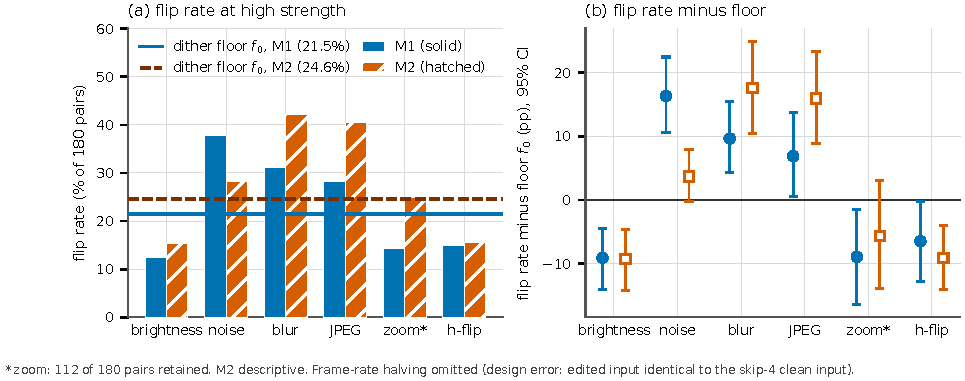
\includegraphics[width=\linewidth]{figures/f1_invariance.pdf}\caption{Flip rate per invariance edit at high strength, with the dither floor as a reference line. The frame-rate edit is a design error and is not interpreted.}\label{fig:f1}\end{figure}}{\par\noindent\textbf{[TODO figure F1: figures/f1\_invariance.pdf missing]}\par}
\IfFileExists{figures/f3_dose.pdf}{\begin{figure}[t]\centering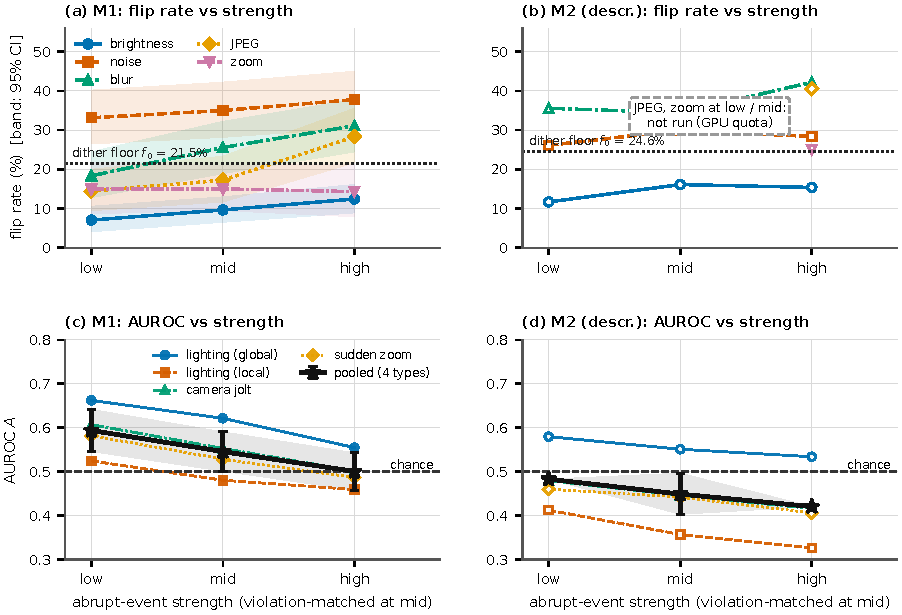
\includegraphics[width=\linewidth]{figures/f3_dose.pdf}\caption{Dose-response for M1: flip rate (invariance edits) and specificity AUROC (abrupt edits) against edit strength. Descriptive.}\label{fig:f3}\end{figure}}{\par\noindent\textbf{[TODO figure F3: figures/f3\_dose.pdf missing]}\par}
